\section{Sonnenoberfläche}
In diesem Abschnitt wird besprochen, wie die Sonnenoberfläche in der Realität
aussieht und wie die Erscheinung prodedural Nachgebildet werden kann. Dabei
wird insbesondere auf die Entwicklung eines entsprechenden CG-Shaders
eingengangen. Grundsätzlich besteht die Möglichkeit, eine Textur zu
generieren, diese in eine Datei zu speichern und anschließend auf das Mesh zu
übertragen. Dies hat jedoch den Nachteil, dass die Textur nur unter sehr
hohem Aufwand über die Zeit verändert werden kann. Deshalb soll die
Oberflächentextur im Shader selbst erzeugt werden, sodass diese in Echtzeit
animiert werden kann. Auch wird das Verfahren erläutert, wie die
Sonnengeometrie erzeugt wird und für den Shader vorbereitet wird.

\subsection{Generierung der Geometrie} 
Bevor eine Textur für die Sonne dargestellt werden kann, müssen zuerst alle
Rahmenbedingungen stimmen. Dies beinhaltet vor allem die Vorbereitung eines
geeigneten Meshes für die Sonnenoberfläche. Im Folgenden wird der Algorithmus
vorgestellt, welcher eine homogene Geometrie für die Sonne erstellt. Dieser
erstellt in erster Linie die Eckpunkte einer Icosphere. Eine Icosphere
besitzt 20 Dreiecke bestehend aus 12 Eckpunkten, welche die Grundlage für
weitere Unterteilungsschritte sind. Dementspreched müssen diese initial
berechnet werden. Anschließend startet der eigentliche Algorithmus zum
Unterteilen der Flächen in kleinere Flächen. Dieser berechnet auf jeder Kante
eines Dreiecks einen Mittelpunkt, sodass für jede Dreiecksfläche insgesamt
drei neue Eckpunkte entstehen. Anschließend müssen die neu erzeugten Punkte
auf die Einheitskugel abgebildet werden, indem die Positionsvektoren
normalisiert werden. Algorithmus \ref{alg:icosphere} soll diesen Vorgang
verdeutlichen.

\begin{algorithm}
  \caption{Unterteilen von Dreiecksflächen auf einer Icosphere}
  \label{alg:icosphere}
  \SetAlgoLined

  \SetKwInOut{Input}{Eingabe}\SetKwInOut{Output}{Ausgabe}

  \Input{Flächen des Basismeshes $M$, Rekursionslevel $n$}
  \Output{Mesh einer Icosphere mit unterteilten Flächen}
  \BlankLine
  \For{$i\leftarrow 0$ \KwTo $n$}{
    $M'\leftarrow \{\}$\;
    \BlankLine
    \ForEach{$d \in M$}{
      $(\vec{a},\;\vec{b},\;\vec{c})\leftarrow d$\;
      \BlankLine
      $\vec{a}'\leftarrow$ calculateMiddlePoint($\vec{a}$, $\vec{b}$)\;
      $\vec{b}'\leftarrow$ calculateMiddlePoint($\vec{b}$, $\vec{c}$)\;
      $\vec{c}'\leftarrow$ calculateMiddlePoint($\vec{c}$, $\vec{a}$)\;
      \BlankLine
      append($M'$, $(\vec{a},\;\vec{a}',\;\vec{c}')$)\;
      append($M'$, $(\vec{b},\;\vec{b}',\;\vec{a}')$)\;
      append($M'$, $(\vec{c},\;\vec{c}',\;\vec{b}')$)\;
      append($M'$, $(\vec{a}',\;\vec{b}',\;\vec{c}')$)\;
    }
    \BlankLine
    $M\leftarrow M'$\;
  }
\end{algorithm}

\begin{figure}
  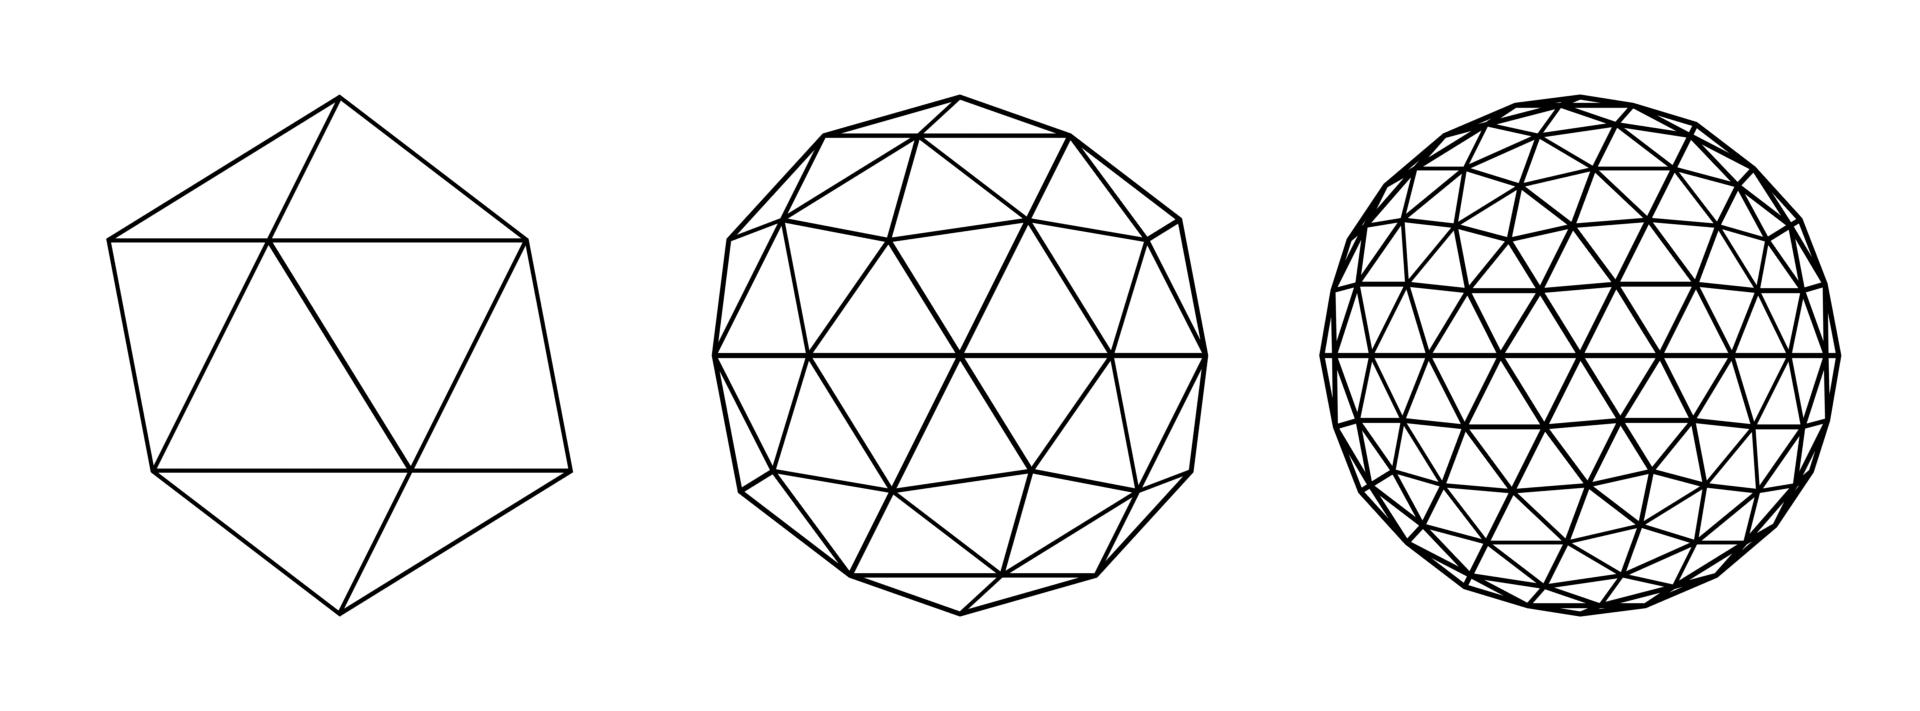
\includegraphics[width=\columnwidth]{icosphere-algorithm}
  \caption{Vergleich zwischen unterschiedlichen Rekursionslevel von Algorithmus \ref{alg:icosphere}. Links befindet sich das Basismodell, in der Mitte die erste und rechts die zweite Rekursionsstufe.}
  \label{fig:icosphere-levels}
  \Description[]{}
\end{figure}

\subsection{Fractal Brownian Motion}
Eine Textur zu erzeugen, die zu jeden Zeitpunkt gleich aussieht wirkt oft
langweilig und uninteressant. Auch, wenn man das Vorbild dieser Arbeit
betrachtet -- die Sonne --, unterscheidet sich die Oberfläche zu jedem
Zeitpunkt von einer vorherigen Messung. Um ein solchen Phänomen zu
modellieren, bedient man sich häufig dem Rauschen. Rauschen hat für
unterschiedliche Fachgebiete eine unterschiedliche Bedeutung. Musiker
verbinden damit störende Geräusche und Astrophysiker denken dabei an
kosmische Hintergrundstrahlung \cite{bookofshaders}. In der Computergrafik
versucht man hingegen, dieses Rauschen künstlich zu generieren, um
beispielsweise eine Textur prozedural zu erzeugen. Auch in dieser Arbeit soll
die Oberflächentextur der Sonne durch ein künstliches Rauschen erzeugt und
verändert werden. Dies entspricht natürlich nicht der Realität, denn die
Sonnenoberfläche hängt von vielen Faktoren, wie der Temperatur und dem
Magnetfeld der Sonne ab. Auch kann man sogenannte Sonnenflecken beobachten,
welche sich als dunkle Flecken auf der Oberfläche äußern. Diese sind nicht
wirklich schwarz, sondern erscheinen dunkler als ihre Umgebung, da diese
Stellen niedrigere Temperaturen aufweisen.

Anstatt nun zu versuchen, die Oberfläche der Sonne so realitätsgetreu wie
möglich nachzubilden, wird in diesem Projekt versucht, mithilfe von künstlich
erzeugtem Rauschen eine ähnliche Oberfläche zu generieren. Hierfür wird, wie
der Titel des Abschnitts andeutet, \textit{Fractal Brownian Motion} verwendet.
Oft werden hierbei Begriffe wie \textit{Oktaven}, \textit{Porosität} und
\textit{Zuwachs} genannt. Eine Oktave beschreibt eine Summe aus mehreren
Rauschfunktionen, die Porosität die Multiplikation der Frequenz um einen konstanten
Wert und der Zuwachs die Verringerung der Amplitude. Algorithmus \ref{alg:fbm} zeigt
ein einfaches zweidimensionales frakturiertes Rauschen basierend auf \cite{bookofshaders}.

\begin{algorithm}
  \caption{Fractal Brownian Motion im zweidimensionalen Raum}
  \label{alg:fbm}
  \SetAlgoLined

  $octaves\leftarrow 1$\;
  $lacunarity\leftarrow 2$\;
  $gain\leftarrow 0.5$\;
  \BlankLine
  $amplitude\leftarrow 0.5$\;
  $frequency\leftarrow 1$\;
  \BlankLine
  \For{$i\leftarrow 0$ \KwTo $octaves$}{
    $y = y + \text{amplitude} * \text{noise}(\text{frequency} \cdot x)$\;
    $\text{frequency} = \text{frequency} \cdot \text{lacunarity}$\;
    $\text{amplitude} = \text{amplitude} \cdot \text{gain}$\;
  }
\end{algorithm}

\subsection{Entwicklung eines Shaders}
